% Chapter 3
\chapter{Proposed Approach} % Write in your own chapter title
\label{Chapter 3}
\lhead{Chapter 3. \emph{Proposed Approach}} % Write in your own chapter title to set the page header
In this chapter we present our proposed scoring system for evaluating subgraphs. We also discuss the feature selection algorithm and classification algorithm which will use the proposed score to classify graphs. 
%\section{Introduction}
%
%\section{Terminologies}
%
%\section{Problem Definition and Solution Methodology}
%
\section{Problem Definition}
%
This paper address the problem of infrequent weighted itemset mining from a transaction dataset. Let {\it I} = \{{\it i1, i2. . . . . ,im}\} a set of data items. Transactional dataset {\it T} =\{{\it t1, t2, t3 . . . . . ,tn}\} is a set of transaction where each transaction is a set of items in {\it I} and denoted by transaction ID (tid). 

An Item set is a set of data items i.e. in {\it k} item sets there is {\it k} items.  Support for an item is the count of that item in the dataset. Based on support count, an item may be frequent or infrequent. For identify an item as frequent or infrequent, a threshold {\it E} is used. This threshold can be set based on user interest. In this paper, we are targeting infrequent items. So, we need to discard items that are above the threshold. 

In regular basis, for frequent item set mining, items and transactions are consider in the same way. But [Ref] according to this paper, we also treating each item differently. Here, each item is paired with it’s weight i.e ({\it I,k}), {\it I} is an item contain in the transaction set {\it T}, {\it K} is the weight of the item that signifies the interest/intensity in the transaction.

As we are working on data stream, we need to process data in an efficient manner. To find infrequent itemset mining from a data stream, we can’t perform multiple scan from a data stream. Once the streams flow  through we lose them. To find recent important knowledge from a data stream, Single-pass and sliding window based mechanism [] is required. 

We have adopted similar definitions presented in the previous works (Carter er al., 1997; Barbar and Hamilton, 2000, 2001, 2003; Li et al., 2005a,b). Let {\it I} = \{{\it i1, i2 . . . . . . , im}\} be a set of items and {\it D} be a transaction database \{{\it T1, T2 . . . . . . , Tn}\} where each transaction {\it Ti} ϵ {\it D} is a subset of {\it I}.
%Definition 1: The measure value mv(ip, Tq), represents the weight of an item ip in transaction Tq. For



%

%
\section{Solution Methodology}
%
In this section, We describe the construction process of our tree structure to store the stream data using a single pass. We use ShrFP-Tree (Share-frequent pattern tree) for share-infrequent pattern mining. The header table is maintained to keep an item order in our tree structure. Each entry of a transaction in a header table  explicitly maintains item-id and weight information for each item. Here, weight is the {\it tmv} (transaction measure value) values of items. To facilitate the tree traversals adjacent links are also maintained (not shown in figure for simplicity) in our tree structure.
%
\par Consider the example data stream at Table~\ref{tab:Table} . At first, ShrFP-Tree captures the {\it tmv} values of all items and keep in header table  as weight. After that, we scan each database transaction one by one and then insert in the tree. In our example, first transaction T1 contains four items one of which is 0. If any item’s weight is 0 in the transaction, we will not insert that item in the tree. So, now we have three transactions {\it b,c,d} and insert them in the tree. 
\begin{figure}[ht]
\centering
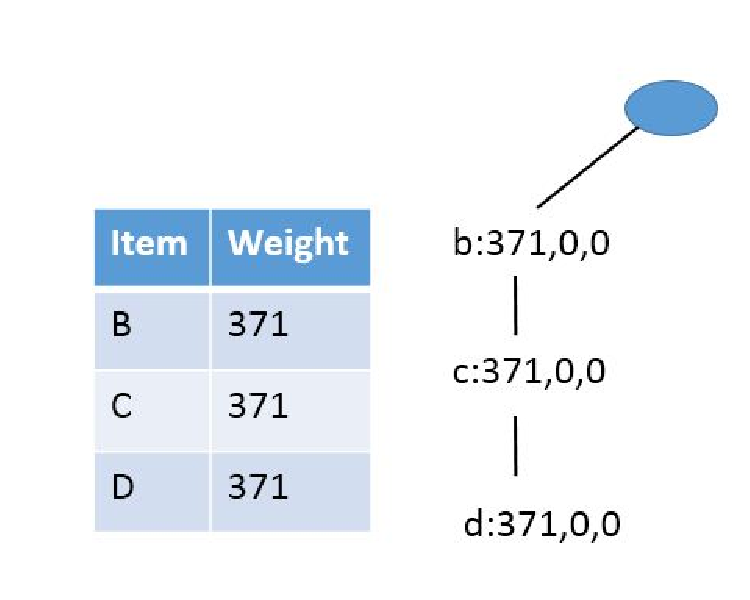
\includegraphics[scale = 0.8] {a.eps}
\caption{After inserting batch 1}
\label{fig:insert1}
\end{figure} 
Figure ~\ref{fig:insert1} shows the tree and header table after inserting batch 1. 
\begin{figure}[ht]
\centering
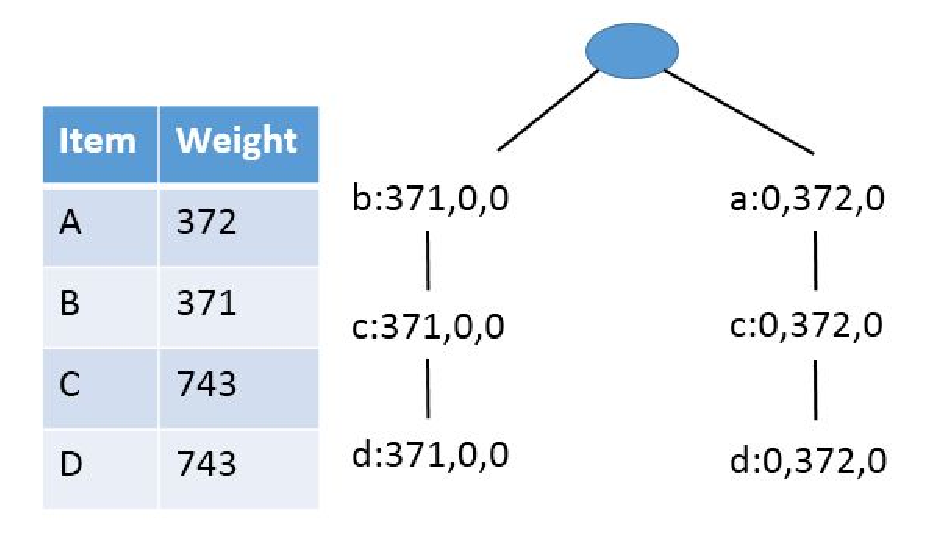
\includegraphics[scale = 0.8] {b.eps}
\caption{After inserting batch 2}
\label{fig:insert2}
\end{figure} 
\begin{figure}[ht]
\centering
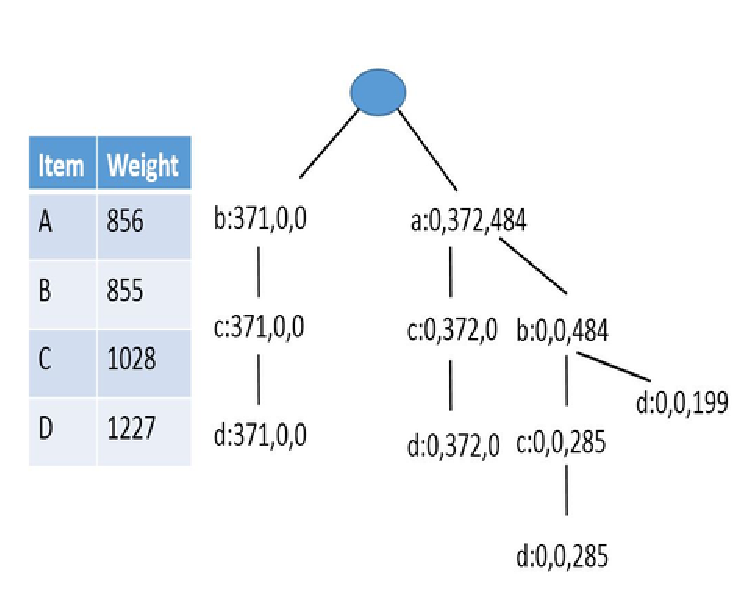
\includegraphics[scale = 0.8] {c.eps}
\caption{After inserting batch 3}
\label{fig:insert3}
\end{figure}
%
\begin{figure}[ht]
\centering
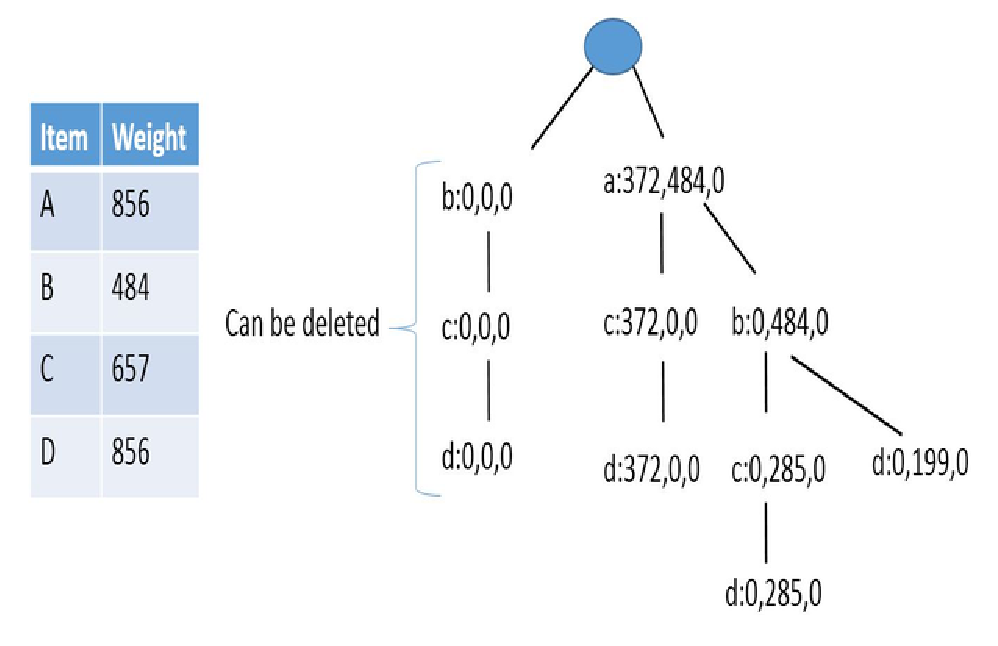
\includegraphics[scale = 0.8] {d.eps}
\caption{Deletion process of batch 1}
\label{fig:insert4}
\end{figure}


\begin{figure}[ht]
\centering
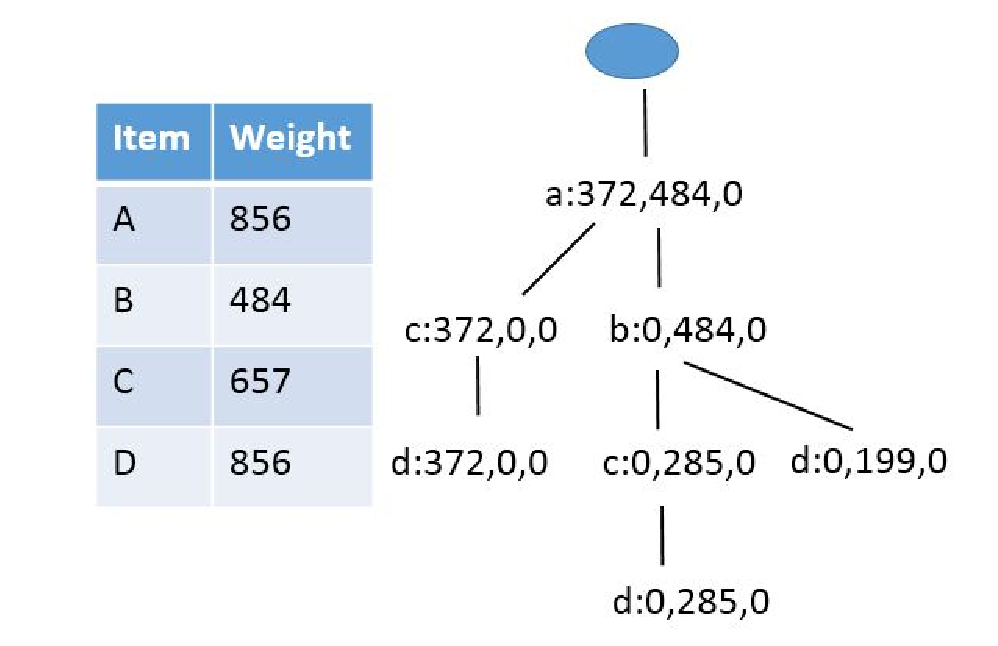
\includegraphics[scale = 0.8] {e.eps}
\caption{After deleting batch 1}
\label{fig:insert5}
\end{figure}


\begin{figure}[ht]
\centering
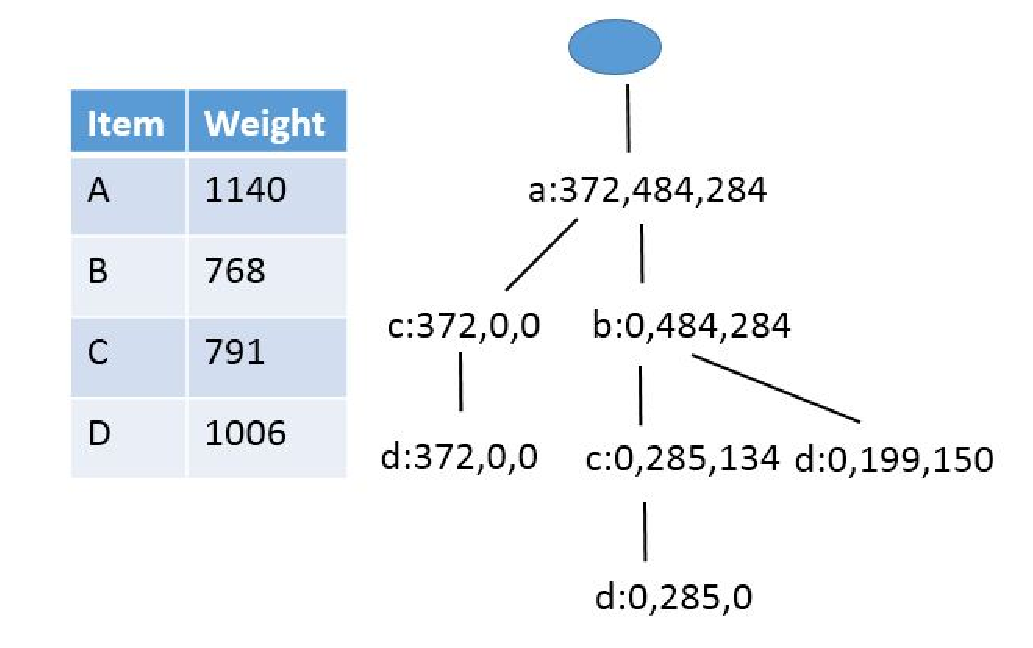
\includegraphics[scale = 0.8] {f.eps}
\caption{After inserting batch 4}
\label{fig:insert6}
\end{figure}
%

\begin{figure}[ht]
\centering
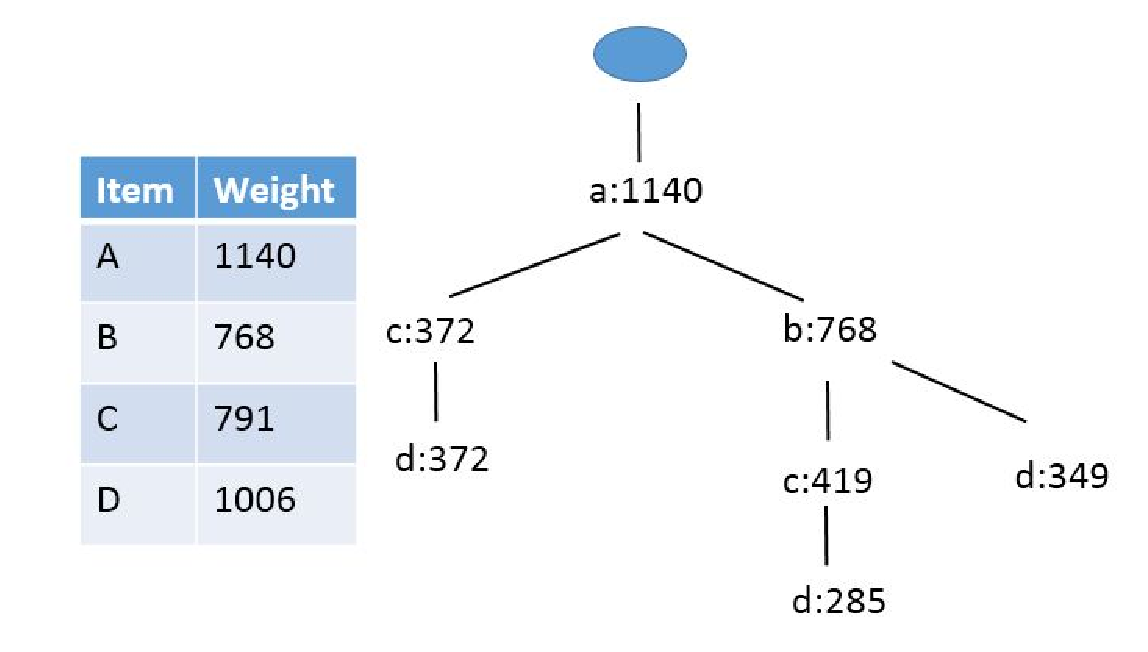
\includegraphics[scale = 0.8] {g.eps}
\caption{Complete tree after inserting window 2}
\label{fig:insert7}
\end{figure}

Figure ~\ref{fig:insert2} shows the tree and header table after inserting batch 2. In the same way, batch 3 also inserted in the tree. The final tree after inserting window 1 in the tree is shown in Figure ~\ref{fig:insert3}.

\par As it’s a data stream, the stream moves to batch 4. It needs to delete previous information of batch 1. Because batch 1 is not belongs to window 2 and therefore the information of batch 1 becomes garbage in the window 2 and it will no longer be used. We delete information of batch 1 from the tree. We also update the header table. After deletion of batch 1, the header table and the tree is shown in Figure ~\ref{fig:insert5}. Some nodes which do not have any information of batch 2 and batch 3. We can delete them from the tree. In case of other nodes, the weight are shifted one position left to remove the weight information of batch 1. Now insert new batch i.e. batch 4 in the tree. As a result, the three weight information of each node represents batch 2, batch 3 and batch 4. Figure ~\ref{fig:insert6} shows the tree after insertion of batch 4.
%
\\*
{\bf Property 1:} The total value of {\it tmv} (transaction measure value) of any node in ShrFP-Tree is greater than or equal to the sum of total value of {\it tmv} values of its children.
\clearpage
\section{Mining Process}
ShrFP-Tree is a pattern growth mining process that mines all the candidate share-infrequent patterns. According to our property 1, pattern growth mining algorithm can be directly applicable to it by using {\it tmv} values.
\par Consider the database of Table~\ref{tab:Table} and maxShare = 0.20 in that database. The final ShrFP-Tree for the database we have considered in Table~\ref{tab:Table}, is shown in Figure ~\ref{fig:insert7}. At first, we have prepared a header table for all items. According to header table, least weighted item will be mined first. In our example, {\it b} is the item for mining. A conditional tree is prepared for item {\it b} is shown in figure(). For preparing conditional tree, we have taken all the branches prefixing the item {\it b}. Based on max{\_}lmv value item {\it b} is not in candidate infrequent pattern list. But its candidate pattern can be in infrequent list. So, we have added them in the candidate infrequent pattern list. Then again, we have started for item {\it c}. Same process is applied for generating conditional tree for item {\it c} shown in figure(). Then we have completed the process for generating candidate infrequent pattern list. Table 2 shows the calculation process for finding actual share-infrequent patterns from the candidate infrequent pattern list. The resultant share-infrequent patterns are \{{\it c}\},\{{\it b,c}\},\{{\it b,c,d}\} for window 2.
\begin{table}
\begin{center}
\begin{tabular}{ |c|c|c|c| } 
\hline
Patterns & lmv & SH & Shared Infrequent Patterns \\
\hline
{\it b} & 235 & 0.206 & No\\
{\it c} & 154 & 0.135 & Yes\\
{\it d} & 357 & 0.313 & No\\
{\it ab} & 486 & 0.426 & No\\
{\it bc} & 171 & 0.152 & Yes\\
{\it ac} & 474 & 0.415 & No\\
{\it cd} & 357 & 0.313 & No\\
{\it bd} & 417 & 0.365 & No\\
{\it abc} & 384 & 0.336 & No\\
{\it acd} & 372 & 0.326 & No\\
{\it abd} & 577 & 0.506 & No\\
{\it bcd} & 199 & 0.174 & Yes\\
{\it abcd} & 285 & 0.251 & No\\


\hline
\end{tabular}
\caption{Calculation process of Share-Infrequent patterns}
\label{tab:Table2}
\end{center}
\end{table}

\clearpage
\section{Proposed Algorithm}
Algorithm will be placed here.
%
%
%\section{Complexity Analysis}
%
%\section{Application of the Proposed Algorithm}
%
%\section{Example Workout}
%

